\documentclass[]{article}
\usepackage{amsmath}
\usepackage{amsthm}
\usepackage{amssymb}
\usepackage{ulem}
\usepackage{graphicx}
\usepackage{tikz}
\usetikzlibrary{matrix,shapes,arrows,positioning,chains}
\usepackage{tkz-base}
\usepackage{tkz-euclide}
\usepackage
[
left=2cm,
right=2cm,
top=2cm,
bottom=2cm,
]
{geometry}

\begin{document}

\newtheorem{problem}{Problem}
\newtheorem{lemma}{Property}

\section{The binary search problem, and its variation}

Here is a git repository of a software. It is known that somewhere in the recent N commits, a bug was introduced, and the task is to efficiently find the commit that introduced the bug.

A well-known solution is to use \texttt{git bash}, i.e. the binary search method: checking the commit at the middle of the commit list, and then depending on the result, checking the commit at the middle of one half parts of the commit list. This is the fastest method under normal conditions.

Now we make a small change to the problem: if the commit to check contains the bug (i.e. it is or is after the first commit introducing the bug), the software would crash the entire computer system during the test and the test has to reboot the computer, which takes five minutes. Testing a software without the bug still takes a short time, say, 30 seconds. In this case, what is the best way to implement the binary search?

One might want to test more "good" commits to avoid time spent on "bad" commits as much as possible. Therefore he would tend to test commits before the middle commit, resulting a test sequence "biased" towards the older commits. In an extreme case, where the bad commits take forever to test, he would just test commits one by one from the oldest commit, until he finds the first commit that crashes the system. Similarly, if a bad commit actually takes less time to test, the binary search would bias towards the newer commits.

Under these conditions, the question is, using the binary search idea, what would be the best commit to test in order to minimize the time cost?

\section{Mathematical formalization}

Let's formalize the question in mathematical languages:

\begin{problem}
	Given a sequence $a_0, a_1, a_2, ..., a_n$, with a number $j$ such that $a_k = 0, \forall k < j$ and $a_k = 1, \forall k \ge j$. $j$ is a random number evenly distributed among integers $1, 2, ..., n$. To get the value of $a_k$, some time is taken. The time cost is $s$ if $a_k = 0$, or $t$ if $a_k = 1$. What is the best method to find $j$ with minimal expectation of total time cost?
\end{problem}

and with some assumption clarified:
\begin{itemize}
	\item The values $a_0 = 0$ and $a_n = 1$ are already known and no need to test. Their existence in the problem is to simplify the numbering system in the solution.
	\item Testing cannot be done in parallel. One cannot start another test until the previous test is finished.
	\item Only testing takes time. Other step is assumed done instantly.
	\item One may get the result by noticing one test takes a longer time before producing the result. However, getting the result in advance does not shorter the time taken by the test, not even for the final step. The total time cost includes the final "rebooting" time even if one already knows the answer.
\end{itemize}

\section{Testing procedure}

The binary-search-like method is illustrated in the chart below.

\tikzstyle{decision} = [diamond, draw, fill=blue!20, 
text width=4.5em, text badly centered, node distance=3cm, inner sep=0pt]
\tikzstyle{block} = [rectangle, draw, fill=blue!20, 
text width=5em, text centered, minimum height=4em, node distance=3cm]
\tikzstyle{line} = [draw, -latex']
\tikzstyle{cloud} = [draw, ellipse,fill=red!20, node distance=2cm,
minimum height=2em]

\begin{tikzpicture}[auto]
\node [cloud](start){start};
\node [block, below of=start](init){set $p = 0$, $q = n$};
\node [decision, below of=init](exit){$p - q = 1$?};
\node [block, below of=exit](choose){$(*)$choose integer $x$ such that $p < x < q$};
\node [decision, below of=choose](test){test $a_x$};
\node [block, left of=test](a){set $p=x$};
\node [block, right of=test](b){set $q=x$};
\node [block, right of=exit](final){set $j=q$};
\node [cloud, below of=final](end){end};

\path [line] (start) -- (init);
\path [line] (init) -- (exit);
\path [line] (exit) -- node {no} (choose);
\path [line] (choose) -- (test);
\path [line] (test) -- node {0, $+s$} (a);
\path [line] (test) -- node {1, $+t$} (b);
\path [line] (a) |-([xshift=-0.5cm,yshift=-0.5cm]a.south west)|- (exit);
\path [line] (b) |-([xshift=-0.5cm,yshift=-0.5cm]a.south west)|- (exit);
\path [line] (exit) -- node{yes} (final);
\path [line] (final) -- (end);

\end{tikzpicture}

\section{The equation}
 
The step $(*)$ is the only place we need to decide how to do exactly. It can be seen that on each iteration, the algorithm is effectively solving the same problem with a smaller size where $n = p - q$, therefore we can choose x by some function $w(n, s, t)$ as
\[
x = w(p - q, s, t) + p \,,
\]
and the expectation of total time $F_{s,t}(n)$ can be expressed recursively as
\begin{equation}
F_{s,t}(n) = \frac{w}{n}(t + F_{s,t}(w)) + \frac{n-w}{n}(s + F_{s,t}(n-w))\,,
\end{equation}
where $w = w_{s,t}(n)$ represents the offset of the next testing point relative to the start of the current range. The two term represents the two possibility where the next iteration goes to the left or the right. Their probability are $\frac{w}{n}$ and $\frac{n-w}{n}$, respectively, based on the assumption of the uniform distribution. $t$ and $s$ are the time cost of the current iteration, and $F(...)$ are the time cost of the rest iteration.

Our goal is to find the most efficient method, so we want to minimize the value of $F(n)$. Therefore, with an initial value $F(1) = 0$, we can define a calculable function $F(n)$ over $n \in \mathbb{Z}$ as
\begin{align*}
F_{s,t}(1) &= 0\,,\\
F_{s,t}(n) &= \min_{0<w<n}^{w\in\mathbb{Z}}\left\{\frac{w}{n}(t + F_{s,t}(w)) + \frac{n-w}{n}(s + F_{s,t}(n-w))\right\} \textrm{ for } n > 1 \,.
\end{align*}

To simplify further analysis, we define the ``normalized" function $E(n) = nF(n)$, which satisfies the following recursive relation
\begin{align*}
E_{s,t}(1) &= 0\,,\\
E_{s,t}(n) &= \min_{0<w<n}^{w\in\mathbb{Z}}\{E_{s,t}(w) + E_{s,t}(n-w) + wt +(n-w)s\} \textrm{ for } n > 1 \,.
\end{align*}

Now let's analyze the function $E_{s,t}(n)$, which represents the expected time scaled by $n$, and the optimizer $w = w_{s,t}(n)$, which represents which commit you should test next given parameters $(n,s,t)$.

\section{Properties}
\hspace{1cm}
\begin{lemma} Homogeneity of $s$ and $t$. For any $k\in\mathbb{R}^+$ we have
\[
	E_{ks,kt}(n) = k E_{s,t}(n)
\]
\[
	w_{ks,kt}(n) = w_{s,t}(n)
\]
This means it is only the ratio $s/t$ that affects the bisecting strategy.
\end{lemma}
\begin{proof}
		Proof by induction. 
	\paragraph{Base case} for $n = 1$, $E_{ks,kt}(1) = 0 = k\cdot0 = kE_{s,t}(1)$
	\paragraph{Inductive step} Assuming $E_{ks,kt}(m) = k E_{s,t}(m)$ holds for all $m = 1,2,\dots,n-1$, we can show that $E_{ks,kt}(n) = k E_{s,t}(n)$ by 
	\begin{align*}
	E_{ks,kt}(n) &= \min_{w}\{E_{ks,kt}(w) + E_{ks,kt}(n-w) + wkt +(n-w)kst\}\\
	  &= \min_{w}\{k E_{s,t}(w) + k E_{s,t}(n-w) + wkt +(n-w)ks\}\\
	  &= k\min_{w}\{E_{s,t}(w) + E_{s,t}(n-w) + wt +(n-w)s\}\\
	  &=kE_{s,t}(n)
	\end{align*}
	and note that the transformation doesn't affect the choice of $w$.
\end{proof}	

\hspace{1cm}
\begin{lemma} Symmetry of $s$ and $t$:
	\[
		E_{s,t}(n) = E_{t,s}(n)
	\]
	\[
		w_{s,t}(n) + w_{t,s}(n) = n
	\]
Together with previous lemma, this means we only needs to study either $s/t \le1$ or $s/t \ge 1$
\end{lemma}
\begin{proof}
	This can be similarly proved by induction. Omitted.
\end{proof}	

\hspace{1cm}
\begin{lemma}
	The optimizer $w_{s,t}(n)$ outputs a set of $w$. It is not necessarily always a single $w$ that minimize the function
\end{lemma}
\begin{proof}
		This is obvious. We haven't really restricted $w$ to be a single value for given $(n,s,t)$. Multiple $w$ can equally give the minimal result in the $E_{s,t}(n)$ equation. In fact, we will see that this is true for most cases. 
\end{proof}	

\hspace{1cm}
\begin{lemma}
$E_{s,t}(n)$ as a function of $n$ is convex
\end{lemma}
\begin{lemma}
	$w_{s,t}(n)$ is always a simple integer interval $[w_{s,t}^{min}(n), w_{s,t}^{max}(n)]$
\end{lemma}
\begin{lemma}
	If $w^*\in w_{s,t}(n)$, then at least one of the following is true: $w^*\in w_{s,t}(n+1)$, or $w^*+1\in w_{s,t}(n+1)$
\end{lemma}
\begin{proof}
(TODO, currently broken)
we will prove the three properties above together using induction.

First of all, let's formally define the convexity of $E(n)$ which is a discrete function over integer. We define the differential as
\[  
\Delta E(n) = E(n+1) - E(n)
\]
and we say that $E_{s,t}(n)$ is convex on $[1,n]$ if and only if
\[
 \Delta E(m)\le \Delta E(m+1)\quad\forall m = 1,2,\dots,n-2\quad (\text{Proposition } \mathbf{C}_n)
\]

We denote the property about $w$ as
\[
w^*\in w(n) \implies w^* \in w(n+1) \lor w^*+1 \in w(n+1) \quad (\text{Proposition } \mathbf{W}_n)
\]

We also denote $D^w_{s,t}(n) = E_{s,t}(w) + E_{s,t}(n-w) +wt+(n-w)s$ so we have
\[
E(n) = \min_w\{D^w(n)\} = D^{w(n)}(n)
\]
\[
D^{w(n)}(n) \le D^{w(n) - 1}(n)\  (\text{if } w(n) > 1)
\]
\[
D^{w(n)}(n) \le D^{w(n) + 1}(n)\  (\text{if } w(n) < n - 1)
\]
We also have 
\[
D^{w}(n+1) = D^{w} + \Delta E(n-w) +s
\]
\[
D^{w+1}(n+1) = D^{w} + \Delta E(w) +t
\]


\paragraph{Base case}
The first few values of $E(n)$ and $w(n)$ are 
\begin{align*}
&E(1) = 0,\ &&\\
&E(2) = s + t, \ &&w(2) = 1,\\
&E(3) = 2s + 2t + \min\{s, t\}, \ &&w(3) = \{1\}, \{2\},\text{ or }\{1,2\}
\end{align*}
It can be seen that proposition $\mathbf{C}_1$ and $\mathbf{W}_2$ hold.

\paragraph{Inductive step} (a) we will show that $\mathbf{C}_n \implies \mathbf{W}_n$ for $n\ge 2$:

If $w(n) >1$, then we have
\begin{align*}
D^{w(n)}(n+1) &= D^{w(n)}(n) + \Delta E(n-w(n)) +s\\
&\le  D^{w(n) - 1}(n) + \Delta E(n-w(n)) +s \quad &(\text{$D^{w(n)}(n)$ is the smallest among $D^{w}(n)$})\\
&\le  D^{w(n) - 1}(n) + \Delta E(n-(w(n)-1)) +s \quad &(\text{Convexity $\mathbf{C}_{n}$}) \\ 
&=D^{w(n)-1}(n+1)
\end{align*}

If $w(n) < n -1$, then we have
\begin{align*}
D^{w(n)+1}(n+1) &= D^{w(n)}(n) + \Delta E(w(n)) +t \\
&\le  D^{w(n) + 1}(n) + \Delta E(w(n)) +t \quad &(\text{$D^{w(n)}(n)$ is the smallest among $D^{w}(n)$})\\
&\le  D^{w(n) + 1}(n) + \Delta E(w(n) + 1) +t \quad &(\text{Convexity $\mathbf{C}_{n}$}) \\ 
&= D^{w(n)+2}(n+1)
\end{align*}

Also notice that $D^w(n+1)$ is convex over $w=1,\dots,n$ due to convexity $\mathbf{C}_{n}$. The inequalities above shows the relations about four consecutive points at the valley of the convex function:
\[
D^{w(n)-1}(n+1) \ge D^{w(n)}(n+1) \sim D^{w(n)+1}(n+1) \le D^{w(n)+2}(n+1)
\]

We can conclude that at least one of $D^{w(n)}(n+1)$ or $D^{w(n)+1}(n+1)$ is the minimum of $D^w(n+1)$, thus $\mathbf{W}_n$ holds

(b) We then show that:
\[
\Delta E(n)= \begin{cases}
	\Delta E(w(n)) + t \quad(w(n+1) = w(n) + 1)\\
	\Delta E(n-w(n)) + s\quad(w(n+1) = w(n))
	\end{cases} \quad (\text{Proposition $\mathbf{W}_n$ ehhhhhhhh})
\]

\end{proof}



\hspace{1cm}
\begin{lemma}
Fixing $n$ and $s$, $E_{s,t}(n)$ as a function of $t$ is concave 
\end{lemma}
\begin{proof}
Proof by induction. The base case $E_{s,t}(1) = 0$ is concave over $t$. In the recursive equation, all the summation components are concave, and the minimal of concave functions is still a concave function.
\end{proof}

\hspace{1cm}
\begin{lemma}
Fixing $n$ and $s$, $E_{s,t}(n)$ is a piecewise linear function of $t$. The nodes are always at rational points.
\end{lemma}
\begin{proof}
	This can be proved by induction. Omitted.
\end{proof}
With this property, we can graph the function with a series of segments. For example, the graph of $E_{1,t}(10)$ over $t\in[0,1]$ is 


	\begin{tikzpicture}[scale=0.8]
	\tkzInit[xmin=0,ymin=0,xmax=1.1,ymax=35,xstep=0.1,ystep=5]
	\tkzDrawX[label={$t$}]
	\tkzLabelX[step=1]
	\tkzDrawY[label={$E_{1,t}(10)$}]
	\tkzLabelY[step=10]
	\tkzDefPoint(0,9){p1}
	\tkzDefPoint(1/8,117/8){p2}
	\tkzDefPoint(1/6,97/6){p3}
	\tkzDefPoint(1/5,86/5){p4}
	\tkzDefPoint(1/3,62/3){p5}
	\tkzDefPoint(1/2,49/2){p6}
	\tkzDefPoint(1,34){p7}
	\tkzDefPoint(1.1,35.5){p8}
	\tkzDrawSegment(p1,p2)
	\tkzDrawSegment(p2,p3)
	\tkzDrawSegment(p3,p4)
	\tkzDrawSegment(p4,p5)
	\tkzDrawSegment(p5,p6)
	\tkzDrawSegment(p6,p7)
	\tkzDrawSegment(p7,p8)
	\tkzDrawPoints(p1,p2,p3,p4,p5,p6,p7)
	\tkzLabelPoint[right](p1){\tiny $(0,9)$}
	\tkzLabelPoint[right](p2){\tiny $(1/8,117/8)$}
	\tkzLabelPoint[right](p3){\tiny $(1/6,97/6)$}
	\tkzLabelPoint[right](p4){\tiny $(1/5,86/5)$}
	\tkzLabelPoint[right](p5){\tiny $(1/3,62/3)$}
	\tkzLabelPoint[right](p6){\tiny $(1/2,49/2)$}
	\tkzLabelPoint[right](p7){\tiny $(1,34)$}
	\end{tikzpicture}

We omitted the graph beyond $t=1$, but remember that it can be derived by $E_{1,t}(n) = t\cdot E_{1,1/t}(n)$ due to symmetry and homogeneity.

It can be seen from the graph that nodes are generally at $t = 1/p$ with some integer $p$. This isn't always true for larger $n$, but computation shows that most nodes are at simple ratios like these.

\hspace{1cm}
\begin{lemma}
	Fixing $n$ and $s$, $w_{s,t}(n)$ is a ``piecewise constant" function. Over a single segment of the piecewise function $E_{s,t}(n)$, the same set of $w$ is chosen. However, at node of piecewise function $E_{s,t}(n)$, $w_{s,t}(n)$ can take a unique value that's not equal to either the left segment or the right segment.
\end{lemma}
\begin{proof}
	Remember that $E_{s,t}(n)$ calculated by taking the $t$-pointwise minimum of a sequence of piecewise linear, convex functions $J_w(t) = E_{s,t}(w) + E_{s,t}(n-w) + wt +(n-w)s$ indexed by $w$. If the pointwise minimum results in a simple linear function over an $t$-interval, it must be resulted from the same set of $w$. This is because, if any $J_w(t)$ tries to join or leave $E_{s,t}(n)$ midway in the interval, it must bend down due to convexity, and that would result in  $E_{s,t}(n) \le J_w(t)$ bending down as well, contradicting with the fact that $E_{s,t}(n)$ is a simple linear function in this interval. $J_w(t)$ can only join or leave at the nodes of $E_{s,t}(n)$
\end{proof}

If we graph $w$ over $t$, we will get a series of ``blocks", separated by vertical lines (marked red) at the nodes of $E$ over $t$. For example, the graph of $w_{1,t}(10)$ over $t\in[0,1]$ is 

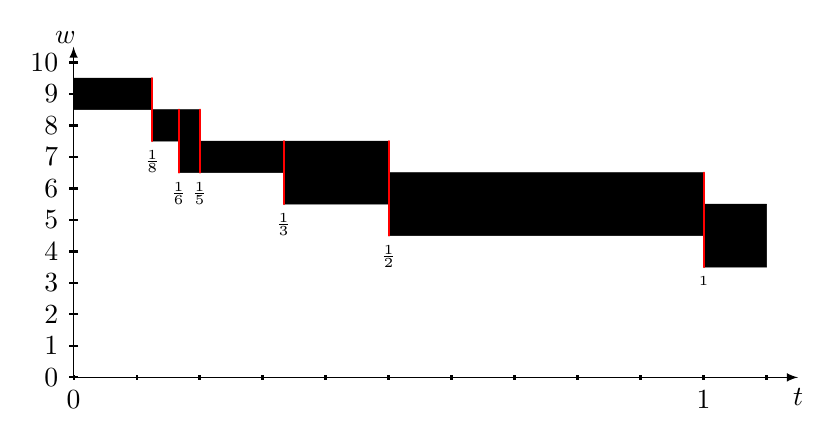
\begin{tikzpicture}[xscale=0.8,yscale=0.4]
\tkzInit[xmin=0,ymin=0,xmax=1.1,ymax=10,xstep=0.1,ystep=1]
\tkzDrawX[label={$t$}]
\tkzLabelX[step=1]
\tkzDrawY[label={$w$},above]
\tkzLabelY[step=1]
\tkzDefPoint(0, 8.5){A}\tkzDefPoint(1/8,9.5){C}\tkzDefRectangle(A,C)\tkzGetPoints{B}{D} \tkzDrawPolygon[fill=black](A,...,D)
\tkzDefPoint(1/8, 7.5){A}\tkzDefPoint(1/6,8.5){C}\tkzDefRectangle(A,C)\tkzGetPoints{B}{D} \tkzDrawPolygon[fill=black](A,...,D)
\tkzDefPoint(1/6, 6.5){A}\tkzDefPoint(1/5,8.5){C}\tkzDefRectangle(A,C)\tkzGetPoints{B}{D} \tkzDrawPolygon[fill=black](A,...,D)
\tkzDefPoint(1/5, 6.5){A}\tkzDefPoint(1/3,7.5){C}\tkzDefRectangle(A,C)\tkzGetPoints{B}{D} \tkzDrawPolygon[fill=black](A,...,D)
\tkzDefPoint(1/3, 5.5){A}\tkzDefPoint(1/2,7.5){C}\tkzDefRectangle(A,C)\tkzGetPoints{B}{D} \tkzDrawPolygon[fill=black](A,...,D)
\tkzDefPoint(1/2, 4.5){A}\tkzDefPoint(1,6.5){C}\tkzDefRectangle(A,C)\tkzGetPoints{B}{D} \tkzDrawPolygon[fill=black](A,...,D)
\tkzDefPoint(1, 3.5){A}\tkzDefPoint(1.1,5.5){C}\tkzDefRectangle(A,C)\tkzGetPoints{B}{D} \tkzDrawPolygon[fill=black](A,...,D)
\tkzDefPoint(1/8, 7.5){A}\tkzDefPoint(1/8,9.5){B}\tkzDrawSegment[color=red,thick](A,B)\tkzLabelPoint[below](A){\tiny $\frac{1}{8}$}
\tkzDefPoint(1/6, 6.5){A}\tkzDefPoint(1/6,8.5){B}\tkzDrawSegment[color=red,thick](A,B)\tkzLabelPoint[below](A){\tiny $\frac{1}{6}$}
\tkzDefPoint(1/5, 6.5){A}\tkzDefPoint(1/5,8.5){B}\tkzDrawSegment[color=red,thick](A,B)\tkzLabelPoint[below](A){\tiny $\frac{1}{5}$}
\tkzDefPoint(1/3, 5.5){A}\tkzDefPoint(1/3,7.5){B}\tkzDrawSegment[color=red,thick](A,B)\tkzLabelPoint[below](A){\tiny $\frac{1}{3}$}
\tkzDefPoint(1/2, 4.5){A}\tkzDefPoint(1/2,7.5){B}\tkzDrawSegment[color=red,thick](A,B)\tkzLabelPoint[below](A){\tiny $\frac{1}{2}$}
\tkzDefPoint(1/1, 3.5){A}\tkzDefPoint(1/1,6.5){B}\tkzDrawSegment[color=red,thick](A,B)\tkzLabelPoint[below](A){\tiny $1$}

\end{tikzpicture}

We omitted the graph beyond $t=1$, but remember that it can be derived by $w_{1,t}(n) = n - w_{1,1/t}(n)$ due to symmetry and homogeneity.

In the case of $n=10$, the vertical lines at nodes don't exceed the $w$ range of its adjacent blocks, but this is not always true for larger $n$. Some vertical lines can looks ``spiky", demonstrating a much larger set of $w$ than the adjacent blocks. This also demonstrates the non-monotonicity of $w_{max}$ and $w_{min}$ over $t$, even though the graph generally looks monotonic. 

\hspace{1cm}
\begin{lemma} (Mode $M_0$) The optimizer degenerates at extreme $s/t$ ratio
	\begin{align*}
	E_{s,t}(n) = (n-1)t + \frac{1}{2}n(n-1)s,\quad & w_{s,t}(n) = \{1\},\quad  &\text{for } \frac{t}{s} > n - 2 \\
	E_{s,t}(n) = (n-1)s + \frac{1}{2}n(n-1)t,\quad & w_{s,t}(n) = \{n-1\},\quad  &\text{for } \frac{t}{s} < \frac{1}{n-2}
	\end{align*}
	($w_{s,t}(1)$ isn't well-defined, so we ignore it here)
\end{lemma}
\begin{proof}
	The two statements above are equivalent due to the symmetry property, so we will just prove the first one by induction
	\paragraph{Base case} For $n=1$, we have
	\[
	E_{s,t}(1) = 0 = (1-1)t + \frac{1}{2}\cdot 1 \cdot (1-1) s
	\]
	and for $n=2$, $w_{s,t}(2) = 1$ is the only possible choice, and
	\[
	E_{s,t}(2) = E_{s,t}(1) + E_{s,t}(1) + t + s = t + s = (2-1)t + \frac{1}{2}\cdot 2 \cdot (2-1) s
	\]
	\paragraph{Inductive step} Assuming $E_{s,t}(k) = (k-1)t + \frac{1}{2}k(k-1)s$ holds for all $k = 1,2,\dots n-1$ and $t/s > k - 2$, we can show that, for $t/s > n - 2 > k - 2$:
	\begin{align*}
	E_{s,t}(n) &= \min_{0<w<n}\{E_{s,t}(w) + E_{s,t}(n-w)+wt+(n-w)s\} \\
	&=\min_{0<w<n}\left\{(w-1)t + \frac{1}{2}w(w-1)s + (n-w-1)t + \frac{1}{2}(n-w)(n-w-1)s+wt+(n-w)s\right\}\\
	&=\min_{0<w<n}\left\{ sw^2 + (t-(n+1)s)w + (n-2)t + \frac{1}{2}n(n+1)s \right\}
	\end{align*}
	The function we want to minimize is quadratic, which has the axis 
	\[
		w_{axis} = -\frac{t-(n+1)s}{2s} = \frac{1}{2}\left(-\frac{t}{s} + n+1\right) < \frac{3}{2}
	\]
	The integer $w$ that's the closest to the axis gets the minimal value. We can see that $w=1$ is always the closest to the axis, therefore it minimize the function to
	\[
		E_{s,t}(n)=s + (t-(n+1)s) + (n-2)t + \frac{1}{2}n(n+1)s = (n-1)t + \frac{1}{2}n(n-1)s
	\]
\end{proof}

\hspace{1cm}
\begin{lemma} 
	(Mode $M_1$) For $k = 1,2,\dots$, the optimizer takes value in the following ranges:
	
	\begin{align*}
	&w_{s,t}(n) = \{k\},\quad &\text{ for } \frac{t}{s} \in \left(n - \left(\frac{1}{2}k(k+1) + 1\right), n - \left(\frac{1}{2}k(k+1) - 1\right)\right)\\
	&w_{s,t}(n) = \{k, k + 1\},\quad &\text{ for } \frac{t}{s} \in \left[ n - \left(\frac{1}{2}k(k+3)\right), n - \left(\frac{1}{2}k(k+1) + 1\right) \right]
	\end{align*}
	
	The first equation for $k=1$ overlaps with Mode $M_0$, and the value agrees. And then the two equations specifies the optimizer value for each $t/s$ segments alternately.

	This mode ends at (TODO).
	
	There is also a symmetrical Mode $M_1$ region for small $\frac{t}{s}$ omitted here.
	
\end{lemma}
\begin{proof}
	TODO
\end{proof}

\hspace{1cm}
\begin{lemma} 
	The ``normalized" optimizer $g_{s,t}(n) = w_{s,t}(n)/n$ is similar to a function $g_{s,t}$ that's independent from $n$.
\end{lemma}
\begin{proof}
	This is rather a heuristic observation than a concrete theorem. Consider a continuous version of the original problem:
	\begin{align*}
		E_{s,t}(1) &= 0, \\
		E_{s,t}(x) &= \min_{0<w<x}^{w\in\mathbb{R}}\{E_{s,t}(w) + E_{s,t}(x-w) + wt+(x-w)s\}\text{ for } x\in\mathbb{R}^+
	\end{align*}
	Remember that the traditional bisect problem has a time complexity of $F(n) = E(n)/n \sim O(\log n)$, we can guess that the solution to the functional equation above is in the form
	\[
	E_{s,t}(x) = k_{s,t}x\ln x
	\]
	Substitute this in the equation, we get
	\begin{align*}
	k_{s,t}x\ln x &= \min_{w}\{ k_{s,t}w\ln w + k_{s,t}(x-w)\ln (x-w)+wt+(x-w)s\}
	\end{align*}
	The function to minimize is differentiable, so we can study its derivative
	\begin{align*}
	&\frac{d}{dw} \{ k_{s,t}w\ln w + k_{s,t}(x-w)\ln (x-w)+wt+(x-w)s\\
	&=k_{s,t}(1 + \ln w) - k_{s,t}(1 + \ln(x-w))+t-s\\
	&=k_{s,t}(\ln w - \ln (x-w)) + t -s
	\end{align*}
	The derivative monotonically increases in $0<w<x$ and approaches $\pm \infty$ at each end respectively, so the single minimal value of the original function is at derivative of $0$
	\begin{align*}
	k_{s,t}(\ln w - \ln (x-w)) + t -s &= 0\\
	k_{s,t} &= \frac{s -t }{\ln w - \ln (x-w)}
	\end{align*}
	and we substitute this back and remove the $\min$ operator, we get
	\[
	\frac{s -t }{\ln w - \ln (x-w)} x\ln x =  \frac{s -t }{\ln w - \ln (x-w)}w\ln w + \frac{s -t }{\ln w - \ln (x-w)}(x-w)\ln (x-w)+wt+(x-w)s\,,
	\]
	which can be simplified to 
	\[
	\frac{\ln(w/x)}{\ln(1-w/x)} = \frac{t}{s}\,.
	\]
	If we define the normalized function $g_{s,t} = w/x$, then it is a function that satisfies
	\[
	\frac{\ln g_{s,t}}{\ln(1-g_{s,t})} = \frac{t}{s}\,.
	\]
	The solution is unfortunately not easy to express in a closed form, but we do get a normalized optimizer function $g_{s,t}$ independent from $n$. The optimizer for the discrete problem should be similar to this.
	
	We can also get the coefficient $k_{s,t}$
	\[
	k_{s,t} = \frac{s -t }{\ln w - \ln (x-w)} = \frac{s -t }{\ln g_{s,t} - \ln (1-g_{s,t})} = -\frac{t}{\ln g_{s,t}} = - \frac{s}{\ln(1-g_{s,t})}
	\]
	and the time solution to the discrete problem $E_{s,t}(n)$ should also be similar to $E_{s,t}(n) = k_{s,t}n\ln n$.

\end{proof}

\begin{lemma} 
	The optimizer $w_{s,t}(n)$ forms several regions of ``modes" for different combination of ${n,s,t}$
\end{lemma}
\begin{proof}
	We can plot the graph of real optimizer $w_{s,t}(n)$ against the optimizer for the continuous problem. In the following graph, the horizontal axis from left to right is ratio $r= t/s$ running from $1$ to $10000$ in logarithmic scale, and the vertical axis from up to down is $n$ running from $1$ to $10000$ in logarithmic scale. The color is from the difference $w_{s,t}(n)/n - g_{s,t}$, where $0$ is colored cyan.
	
	\includegraphics[scale=0.18]{w-map.png}\,\includegraphics[scale=0.18]{w-map-marked.png}
	
	We can see the graph is divided into several regions. We have already discussed mode $M_0$ and $M_1$ above. There are also mode $M_2$, $M_3$ and so on. A new mode $M_{n+1}$ is formed when the "short branch" ($E(w)$ when $w$ is small) falls into mode $M_n$. It is anticipated that there are infinitely many $M_n$ modes, but it is hard to verify as their range of $n$ gets exponentially large.
	
	Around $s \approx t$, there is mode $S$, where the graph appears a little bit chaotic.
\end{proof}

%%%%%%%%%%%%%%%%%%%%%%%%%%%%%%%%%%%%%%%%%%%%%%%%%%%%%%%%%%%%%%%%%%%%%%%%%%%%%%%%%%%%%%%%%%%%%%%%%%%%%%%


\section{Back to the classic binary search}
In the original binary search problem is represented by $s = t = T$. In this case, the recursive equation becomes
\[
F_{s,t}(n) = T + \min_{0<w<n}\left\{\frac{w}{n}F_{s,t}(w) + \frac{n-w}{n}F_{s,t}(n-w)\right\}
\]

TODO



\end{document}